\subsection{Attention and Transformer} % 2.5 pages
The attention mechanism originated from the human experience of perceiving things either visually or audibly.
Intuitively speaking, when we observe something through sight, we do not pay attention to all the details but paying attention to a certain part that needs to be focused and giving low attention to the surroundings.

The attention mechanism was firstly added to recurrent neural networks as a visual attention modelling.
In 2014, \citet{mnih2014recurrent} proposed a recurrent attention model that combined ideas in RNN and the attention mechanism for image classification and achieved good performance.
Besides, the researchers discussed and reached forward-looking conclusions that it can be used in object recognition and video classification in future work due to the encouraging results achieved.

In 2016, \citet{bahdanau2016neural} firstly introduced the attention mechanism into the natural language processing field.
In their work, they perform translation and alignment jointly with the attention mechanism on machine translation tasks because ``the use of a fixed-length vector is a bottleneck in improving the performance of this basic encoder-decoder architecture'', said by \citet{bahdanau2016neural}.

\begin{minipage}[]{\textwidth}
\centering
\begin{minipage}[ht]{.35\textwidth}
    \centering
    \begin{figure}[H]
        \centering
        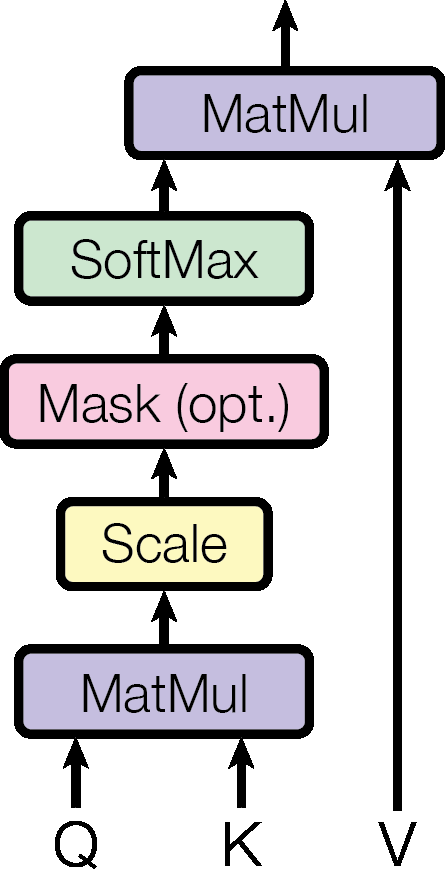
\includegraphics[width=.48\textwidth]{literature/imgs/ext-attention-dot-product.png}
        \caption{Scaled Dot-Product Attention \cite{vaswani2017attention}}
        \label{fig:ext-attention-dot-product}
    \end{figure}
    \vspace*{-.5cm}
    \begin{figure}[H]
        \centering
        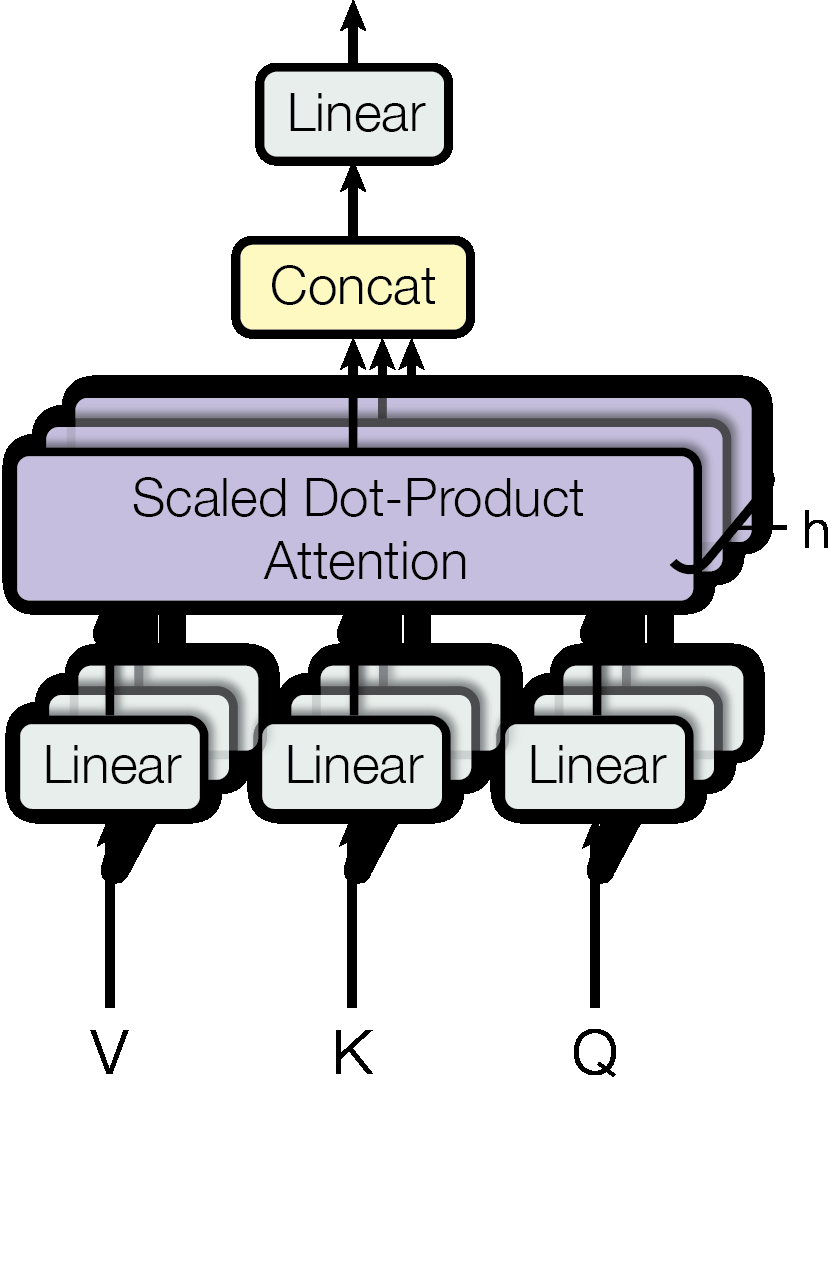
\includegraphics[width=.9\textwidth]{literature/imgs/ext-attention-multihead.png}
        \vspace*{-2em}
        \caption{Multi-Head Attention \cite{vaswani2017attention}}
        \label{fig:ext-attention-multihead}
    \end{figure}
\end{minipage}
\hspace{1em}
\begin{minipage}[ht]{.52\textwidth}
    \begin{figure}[H]
        \centering
        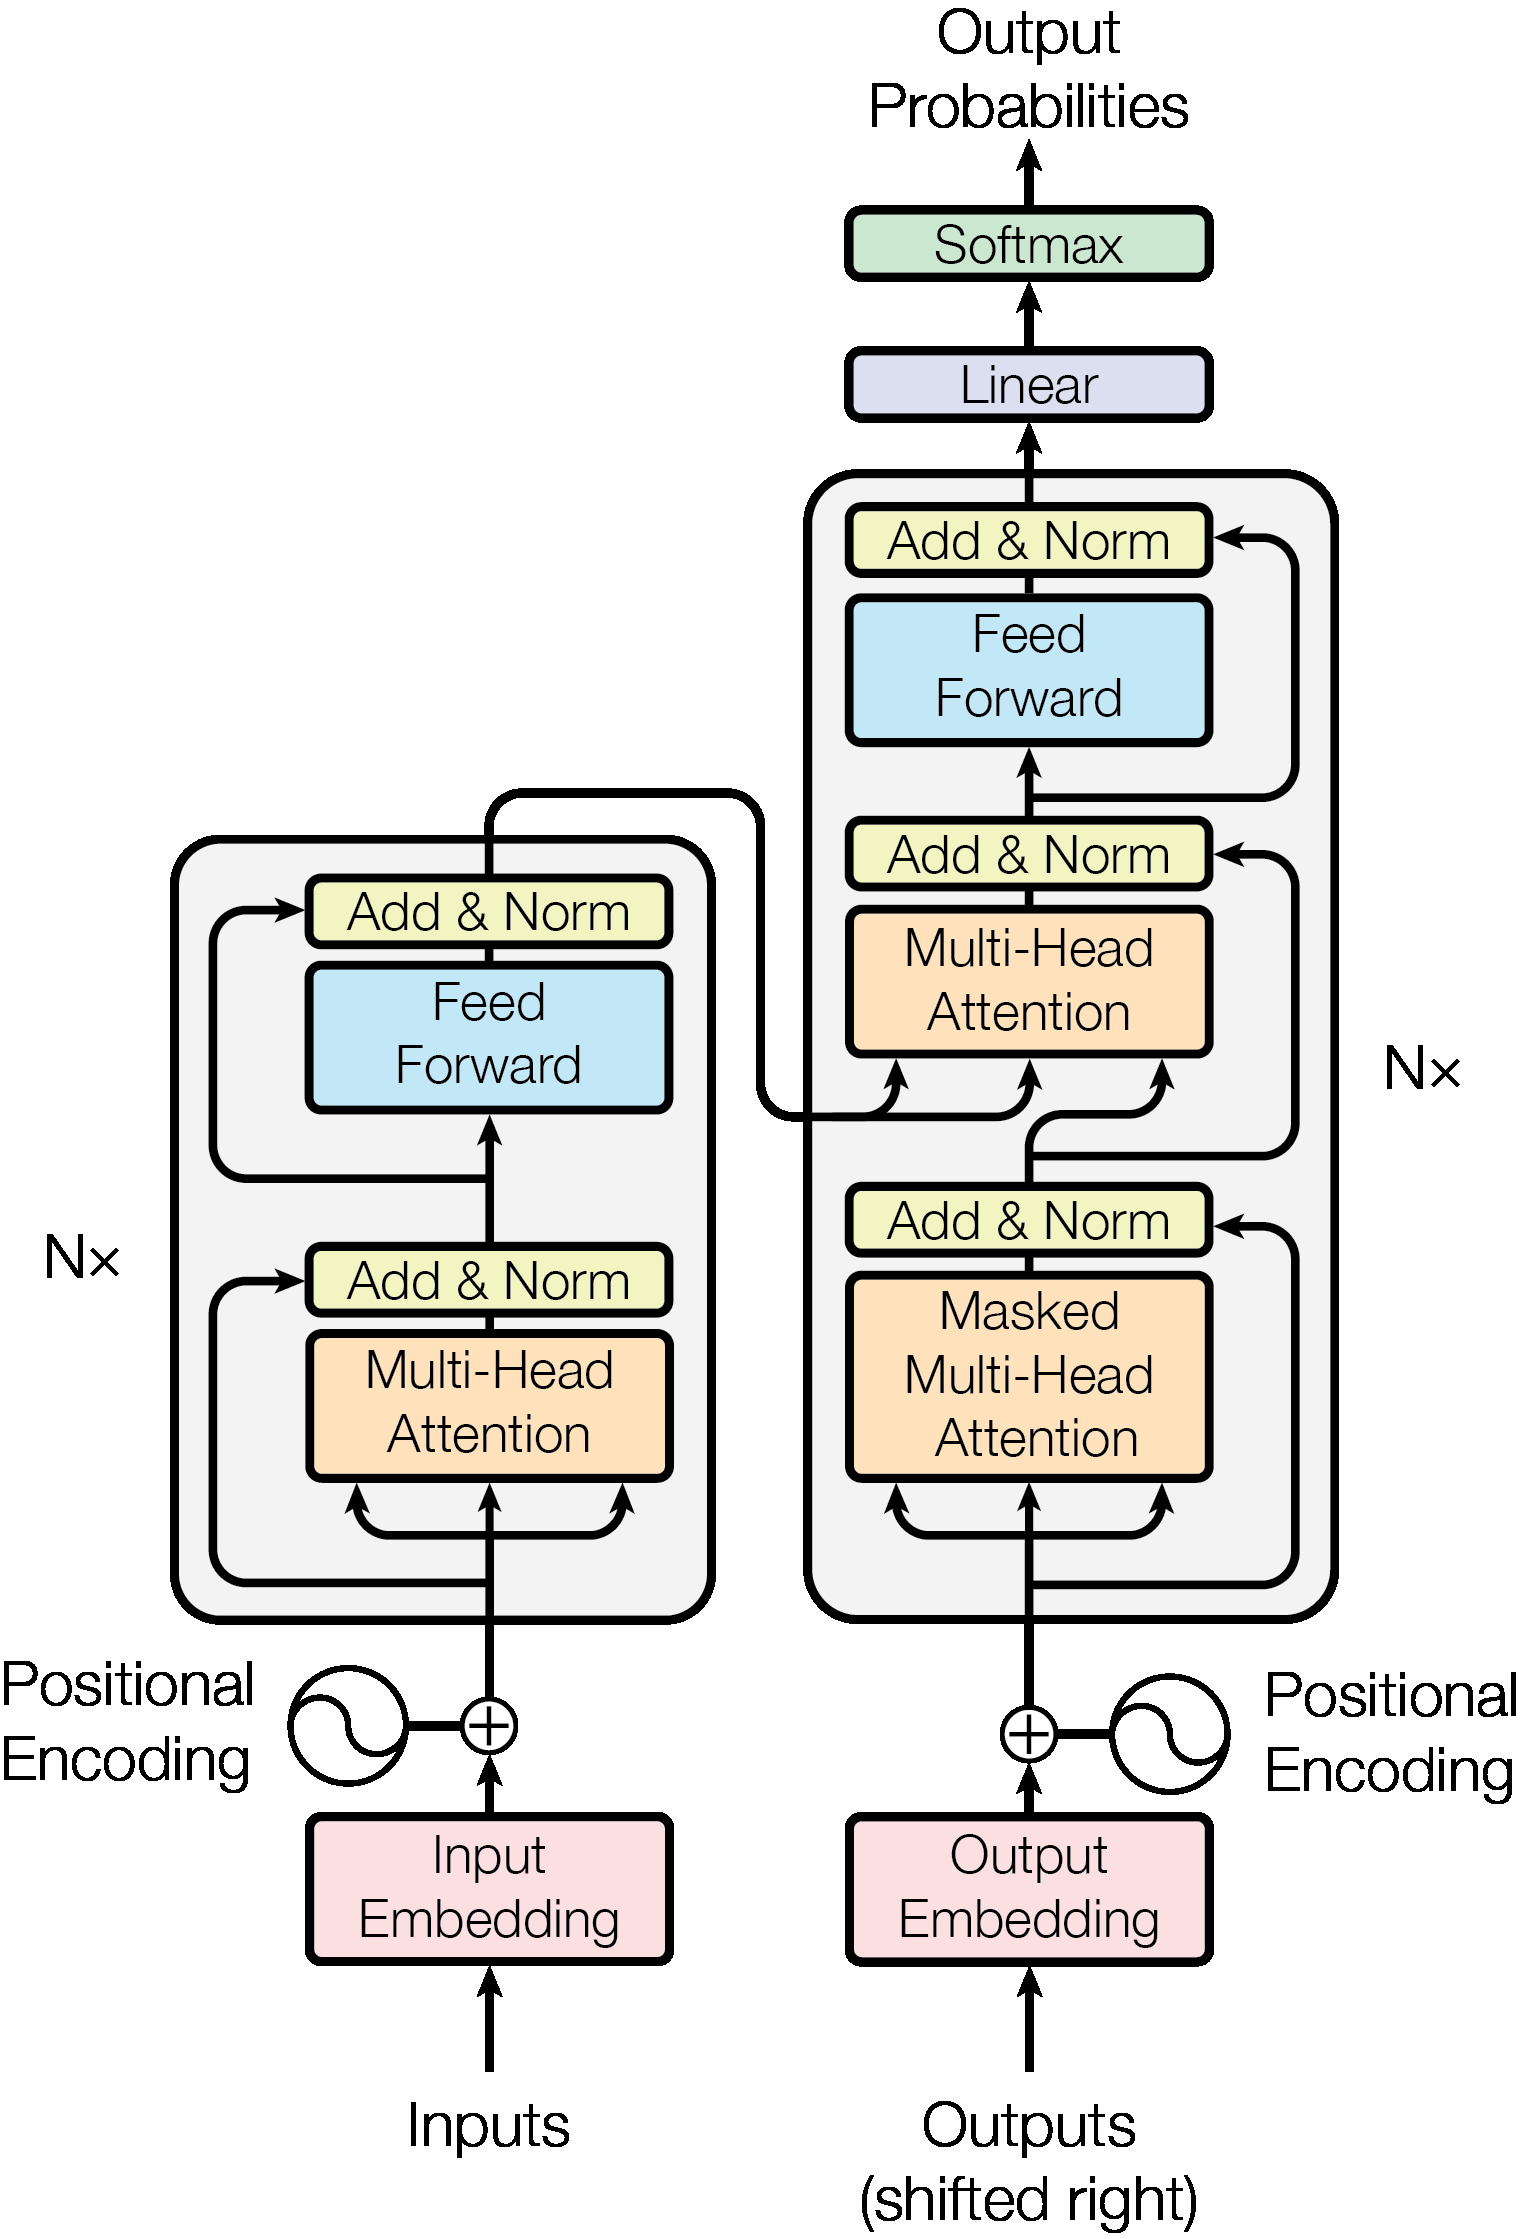
\includegraphics[width=\textwidth]{literature/imgs/ext-transformer.png}
        \caption{The Transformer model architecture \cite{vaswani2017attention}}
        \label{fig:ext-transformer}
    \end{figure}
\end{minipage}
\end{minipage}

One year after the attention mechanism was applied in the machine translation tasks, \citet{vaswani2017attention} proposed scaled dot-product attention (Figure \ref{fig:ext-attention-dot-product}), multi-head attention (Figure \ref{fig:ext-attention-multihead}) and the Transformer model (Figure \ref{fig:ext-transformer}) that is ``relying entirely on self-attention to compute representations of its input and output without using sequence aligned RNNs or convolution'', said by \citet{vaswani2017attention}.
Then, experiments were performed on the machine translation task using the proposed Transformer model and achieved better performance and results, making the attention mechanism the most preferred solution for natural language processing tasks.

\begin{equation}
    Attention(Q, K, V) = softmax(\frac{QK^T}{\sqrt{d_k}})V
    \eqcite{vaswani2017attention}
    \label{equ:2-attention}
\end{equation}

Figure \ref{fig:ext-attention-dot-product} shows the scaled dot-product attention mechanism, where Q, K, and V represent Query, Key and Value respectively.
Further, formula \ref{equ:2-attention} shows the calculation process of it mathematically.
In this formula, the dot-product between Query and Key matrix represents their similarity, which is normalised by the square root of the dimension of $d_k$, since dot-product may grow large in magnitude, pushing the softmax activation function into regions where it has extremely small gradients.
The result from softmax activation is normalised probabilities representing the attention matrix visualised in Figure  \ref{fig:ext-attention_map_portuguese}.

\begin{figure}[!ht]
    \centering
    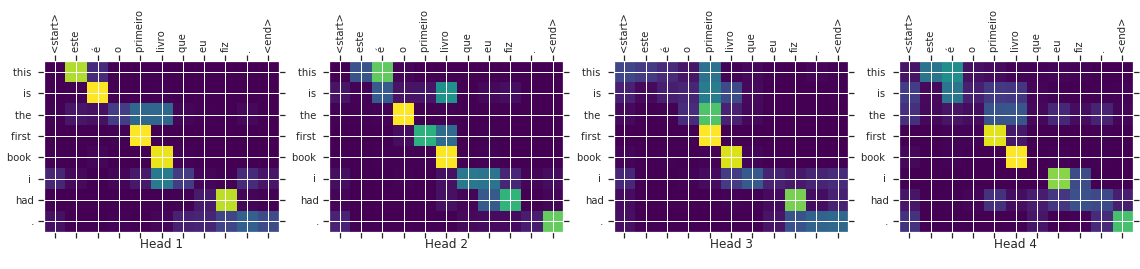
\includegraphics[width=\textwidth]{literature/imgs/ext-attention_map_portuguese.png}
    \caption{Multi-head attention matrix visualisation \cite{tensorflow2021transformer}}
    \label{fig:ext-attention_map_portuguese}
\end{figure}

The idea behinds multi-head attention is like using multiple kernels in CNN to capture different features.

%Transformer
While convolutional neural network (CNN) is in the ascendant among the fields of computer vision, transformer model composed of self-attention structures has achieved state-of-the-art results in many natural language processing tasks.

\citet{devlin2019bert}

The transformer model gradually replaced the recurrent neural network (RRN) with sequential computing restriction and long-term memory loss issues.

Innovative design concepts from the transformer model are also carried forward in the fields of computer vision.

Many recent studies, such as Data-efficient image Transformers (DeiT) and Shifted window (Swin) transformers, have improved widely-adopted CNN-only models such as VGG and ResNet by introducing the self-attention structures to achieve better performance.

\citet{dai2021coatnet}

\citet{guo2021cmt}